\documentclass[UTF8]{ctexart}
\usepackage{main} % 加载自定义样式
\begin{document}

\vspace{80pt}

\title{基于动态规划的穿越沙漠策略}

\maketitle

\begin{center}
    \begin{minipage}{6cm}
        马元昊\:倪皓玥\:曹宇丰
    \end{minipage}
\end{center}

\newpage

\setstretch{1.35}
\begin{abstract}
\zihao{-4}
“穿越沙漠”是一款生存型游戏，需要选择最佳游戏策略，使玩家在保证到达终点的情况下尽可能获得更多资金。
%
针对“穿越沙漠”问题中不同信息条件下的路径规划、资源配置与多人协同行动决策，本文以剩余资金最大化为核心目标，
%
建立了单人确定性决策模型、单人随机决策模型以及多人协同优化模型，对不同关卡情形下的最优策略进行了系统研究。
%
首先，根据地图中各区域的邻接关系构建无向图模型，利用Dijkstra 算法求解起点、村庄、矿山与终点之间的最短路径，
%
为后续策略优化提供路径基础。

对于问题一，我们认为玩家不可能在任意结点停留，因此我们首先证明：除了沙暴天气必须停留以外，玩家只可能在矿山
%
停留挖矿，其余地点不做停留；然后，我们再根据游戏规则，给出玩家向前行走、沙暴时原地停留、矿山挖矿、村庄补给
%
等情况下生活必需品以及资金剩余量的递推关系式的基础之上，以剩余资金最多为目标，设置了玩家按时到达、生活必需
%
品重量不超过负重上限的约束条件，建立了单目标最优化模型，采用动态规划和回溯法，使用$C\mathbin{++}$编程求解。

对于问题二，在仅知道当天天气、未来天气具有随机性的条件下，将天气演化过程引入马尔可夫决策思想，
%
建立基于状态转移概率的动态决策模型。模型结合当前位置、剩余资源、剩余天数及资金状态，
%
给出玩家向前行走、沙暴时原地停留、矿山挖矿、村庄补给等动作进行滚动优化，从而获得不确定天气
%
条件下的最优策略，提高了模型在动态环境中的适应能力。

对于问题三，考虑多人同时参与时因同行、同购和同矿带来的资源消耗放大与收益分摊效应，
%
我们选择合作而非竞争的的博弈模式，在单人模型基础上建立多人协同优化框架。
%
进一步采用蒙特卡洛方法模拟天气过程，对不同随机天气样本下的多人协同行为进行数值实验，
%
从而评估策略的稳定性与收益表现。结果表明，所建模型能够较好统筹路径选择、资源补给与行动安排，
%
在确定与不确定天气条件下均具有较强的适用性与可解释性。

本文提出的模型将最短路径搜索、动态规划、马尔可夫决策与蒙特卡洛模拟有机结合，
%
可为复杂环境下的资源受限路径优化与群体协同决策问题提供参考。

\indent \textbf{关键词：Dijkstra算法；动态规划；马尔可夫决策；蒙特卡洛模拟；路径优化；资源配置}

\end{abstract}

\newpage

\zihao{-4}
\section{问题重述}
\subsection{问题背景}
“穿越沙漠”是一个以资源受限条件下路径规划与决策优化为核心的策略类游戏。
%
玩家需要在给定地图上，从起点出发，穿越沙漠并最终到达终点。
%
游戏过程中，玩家必须合理安排每日行动、购买和消耗水与食物，
%
并结合天气变化、村庄补给和矿山挖矿等机制制定最优策略，以保证在规定期限内完成穿越任务，
%
同时尽可能保留更多资金。具体规则如下：

\begin{figure}[H]
    \centering
    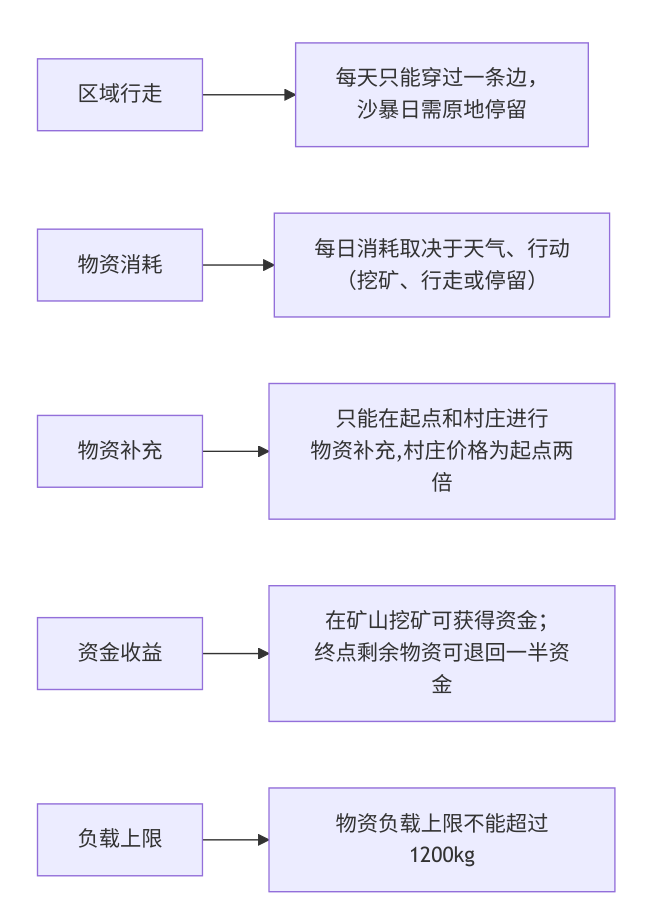
\includegraphics[width=0.7\textwidth]{C2020b/figure/问题背景.png}
    \caption{问题背景}
\end{figure}

此外，在多名玩家的情况下，还存在同行物资消耗翻倍、多人同时挖矿收益压缩等规则。

\subsection{需解决的问题}

根据题目设定，需要针对不同信息条件和参与人数建立相应模型，为玩家制定最优或近优策略，
%
使其在成功到达终点的前提下剩余资金尽可能多。具体需要解决如下问题：

\begin{itemize}
    \item 问题一：单人、天气完全已知情形。
        假设仅有一名玩家参与游戏，且在整个游戏周期内每天的天气状况均已提前知道。
        需要在已知天气序列、地图结构、资源价格、负重上限和截止日期的前提下，
        确定玩家每天的最优行动方案，包括是否移动、是否停留、是否前往村庄补给、是否前往矿山挖矿，
        以及初始阶段应购入多少水和食物，并对附件中的前两关进行求解。
    \item 问题二：单人、天气部分未知情形。
        假设仍只有一名玩家，但玩家仅知道当天的天气，而无法提前获知未来天气状况，
        只能根据当前状态决定当天行动。此时需要建立适用于随机天气环境下的动态决策模型，
        使玩家能够依据当前位置、剩余资源、剩余资金和剩余时间实时调整策略，
        并对附件中的第三关和第四关进行讨论。
    \item 问题三第一问：多人、天气已知情形。
        当有多名玩家同时从起点出发，且天气信息完全已知时，每位玩家的行动方案需在第1天确定后不再改变。
        由于多人同行、同矿和同村补给会引起资源消耗、收益和价格变化，因此需要建立多人协同优化模型，
        确定各玩家应采取的路径与分工策略，并对附件中的第五关进行具体分析。
    \item 问题三第二问：多人、天气部分未知情形。 
        假设多名玩家仅知道当天的天气状况，并且从第2天起，
        所有玩家在每天结束后都可以获知其他玩家当日的行动方案及剩余资源情况，然后再决定下一天的行动。
        这一情形下，玩家之间既存在竞争，也存在一定的信息互动与协同关系。需要建立适用于动态博弈环境的决策模型，
        研究一般情况下玩家应采取的策略，并对附件中的第六关进行讨论。
\end{itemize}
%\subsection{问题背景}

%\subsection{需解决的问题}

\section{问题分析}
\subsection{问题一分析}
在问题一中，玩家需要经过两个关卡，但是其本质都是一致的。
%
玩家需要在遵守游戏规则的前提下，尽可能地多保留资金。
%
于是问题一即为根据参与者在游戏过程中所要满足的各种条件前提下，如何最大化关于资金的函数。
%
我们根据游戏规则，可以依据向前行走、沙暴时原地停留、矿山挖矿、村庄补给等情况，建立关于物资，资金和负重的递推表达式，最后可以化为单目标优化问题。
%
考虑到题目图结构复杂，暴力搜索计算耗时较长，所以我们使用动态规划来求解。

\subsection{问题二分析}
第二问中未来天气未知，题目由确定性优化转化为随机动态决策问题，
%
因此需要在状态转移中引入天气的不确定性，用马尔可夫决策思想描述“当前状态—行动选择—未来状态”的演化过程，
%
使玩家能够依据当天天气和当前资源状况滚动调整策略。
\subsection{问题三分析}
第三问进一步加入多名玩家同时行动时的同行、同矿、同购惩罚，使问题由单人最优扩展为多主体耦合优化问题，
%
不再只追求单条最优路径，而要综合考虑玩家之间的分工、错峰和协同；同时，由于天气过程具有随机性，
%
本文采用蒙特卡洛方法模拟多种天气样本，对多人策略在不同天气实现下的收益与稳定性进行评估。

第五关在天气已知的前提下，分析挖矿收益与需要多消耗物资的关系，确定挖矿亏损，选择直达终点。
%
在次基础上再考虑多人同行惩罚，采用一人停留来换取团队最大总收入，采用合作而非竞争的博弈策略。

第六关对于天气未知情况的三人决策，由于存在同行消耗惩罚和收益惩罚，故也采用合作，让一人挖矿，
%
两人直达的方案进行。通过对天气情况与消耗的分析，确定是否需要补给以及补给次数，
%
最后给出一般情况下的最优路径。

\section{模型假设}
\begin{enumerate}
    \item 不考虑途中资源损耗、丢失及额外获取等特殊情况；
    \item 导致游戏无法进行的极端沙暴天气不会出现；
    \item 除题目说明的价格变化外，不考虑其他额外成本；
    \item 在蒙特卡洛模拟中，各次天气样本相互独立，可视为对真实天气过程的合理近似。
\end{enumerate}

\section{符号说明}
\begin{table}[H]
\centering
\begin{tabularx}{\textwidth}{
  >{\centering\arraybackslash}X  % 符号列：占1/3宽度，居中
  >{\centering\arraybackslash}p{0.667\textwidth}  % 含义列：占2/3宽度，居中
  }
    \toprule[1.5pt]  % 顶部粗线
    \midrule
    符号 & 含义 \\
    \midrule
    $G$ & 剩余金额 \\

$N_t$ & 第$t$日所在区域编号 \\

$\Omega_s = \{N_s\}$ & 起点编号集合 \\

$\Omega_e = \{N_e\}$ & 终点编号集合 \\

$\Omega_v = \{N_{v_i} \mid i\in\mathbb{N}^*\}$ & 村庄编号集合 \\

$\Omega_h = \{N_{h_i} \mid i\in\mathbb{N}^*\}$ & 矿山编号集合 \\

$D$ & 天气（1-晴朗，2-高温，3-沙暴） \\

$X$ & 动向（1-移动，2-停留，3-挖矿） \\

$T = \max t$ & 到终点时的天数 \\

$n$ & 玩家总数 \\

$i\in\{1,2,\dots,n\}$ & 玩家编号 \\

$E$ & 地图邻接边集合 \\

$a_{uv}$ & 邻接矩阵元素，若区域 $u,v$ 相邻则 $a_{uv}=1$，否则 $a_{uv}=0$ \\

$Y_{i,t}^{uv}$ & 第 $i$ 名玩家在第 $t$ 日是否沿边 $(u,v)$ 移动的0-1变量 \\

$Z_{i,t}^{h}$ & 第 $i$ 名玩家在第 $t$ 日是否在矿山 $h\in\Omega_h$ 挖矿的0-1变量 \\

$Q_{i,t}^{v}$ & 第 $i$ 名玩家在第 $t$ 日是否在村庄 $v\in\Omega_v$ 购买资源的0-1变量 \\

$k_t^{uv}$ & 第 $t$ 日沿边 $(u,v)$ 同时移动的玩家数 \\

$k_t^{h}$ & 第 $t$ 日在矿山 $h$ 同时挖矿的玩家数 \\

$k_t^{v}$ & 第 $t$ 日在村庄 $v$ 同时购买资源的玩家数 \\

$\delta$ & 联盟稳定性指标 \\

$\mathcal P_i$ & 由前两问路径模型生成的第 $i$ 名玩家候选可行路径集 \\

$\pi_t(d'\mid d)$ & 天气状态从 $d$ 转移到 $d'$ 的条件概率 \\

$V_t(\cdot)$ & 第 $t$ 日滚动决策价值函数 \\
    \midrule

    \bottomrule[1.5pt]  % 底部粗
\end{tabularx}
\end{table}

\vspace{1em}
\noindent 注：未列出符号及重复的符号以出现处为准

\section{模型的建立与求解}
\subsection{问题1的建模和求解}
根据题意，玩家停留和移动都需要消耗物资，可在起点和村庄购买物资，在矿山处可以挖矿赚取资金，但沙尘暴天气无法前进，最后可以在终点处退还剩余的物资换取资金。
%
玩家需要在30天内从起点出发，最终到达终点，要求最大化最终的金额。梳理题目中的所有要求，画出题目示意图。

\begin{figure}[H] % 参数 h(here), t(top), b(bottom), p(page) 控制浮动位置
    \centering % 使图片居中
    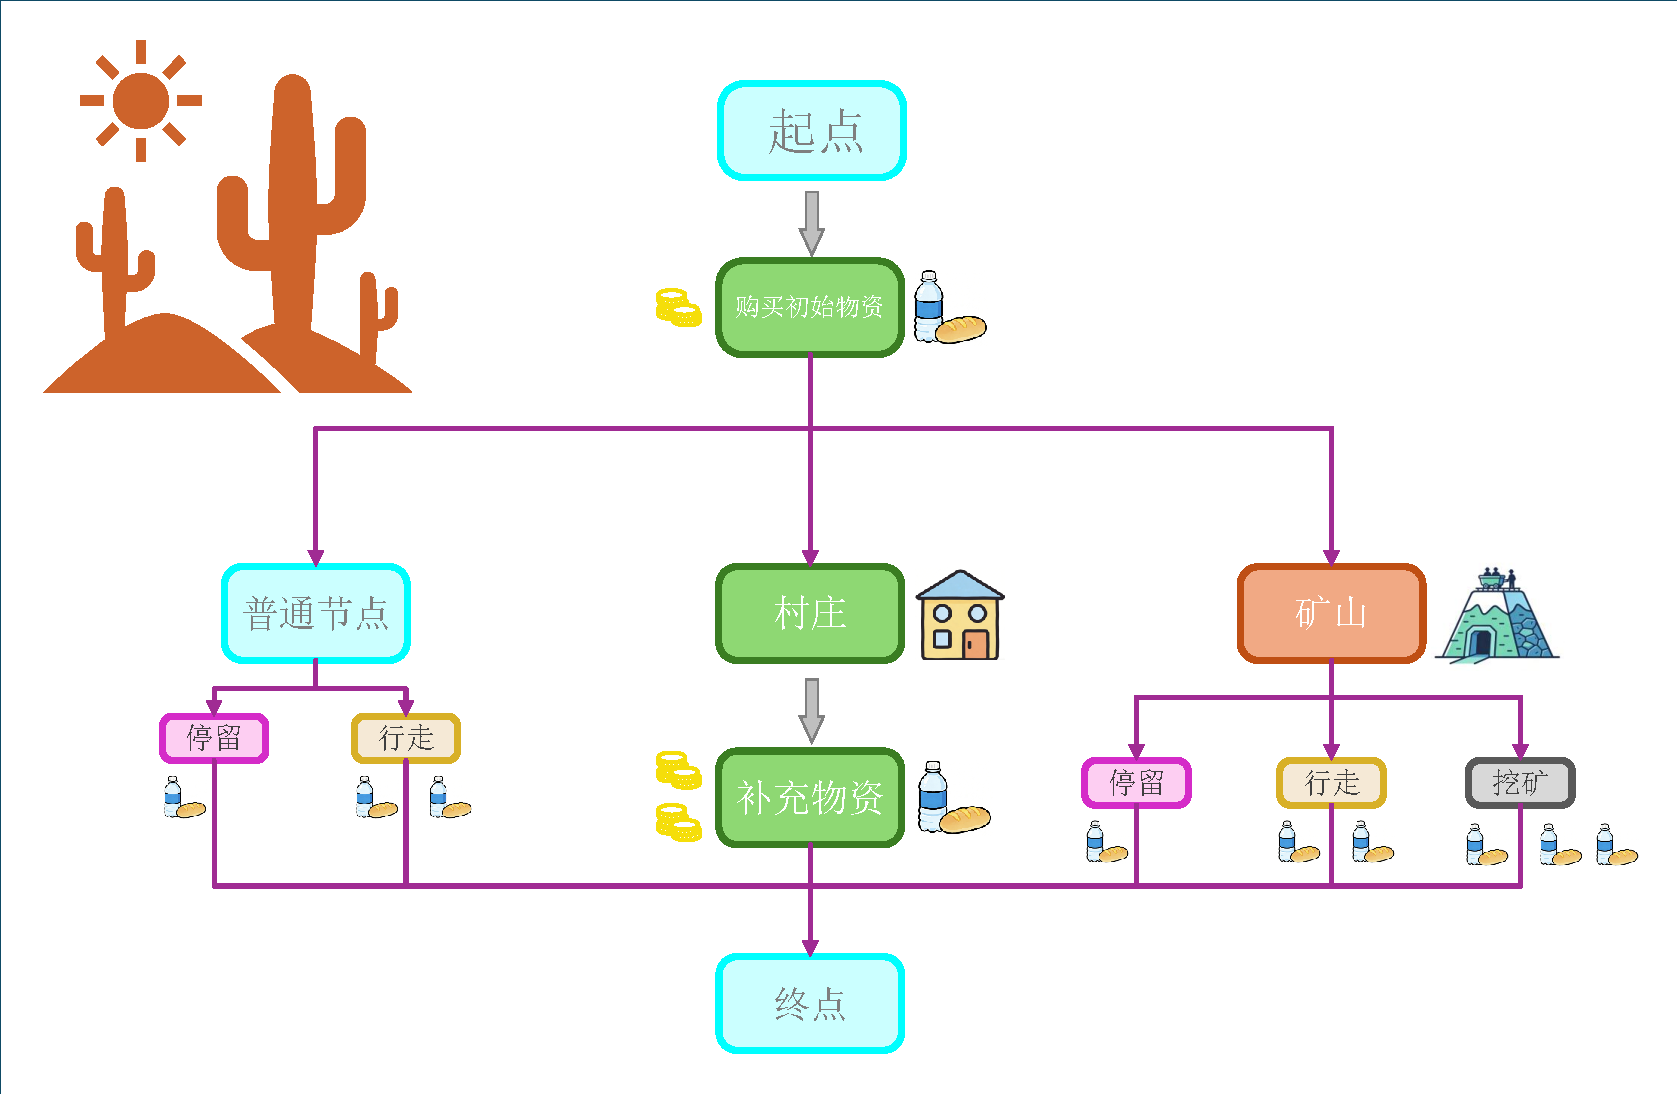
\includegraphics[width=0.8\textwidth]{C2020b/figure/题目示意图.pdf}
    \caption{题目示意图} % 图片标题
\end{figure}

\subsubsection{在已知天气情况时一名玩家的最佳策略模型的建立：}
\noindent\ding{70} \textbf{最简地图模型的建立}：

为了简化后续动态规划的复杂度，我们先对题目所给出的图进行简化，把每个区域看成一个点，把区域相邻的条件看成两个区域之间有一条无向边，由此对地图进行重构。

观察题目可以发现，去往矿山和村庄等重要节点时，在走的天数相同的情况下，消耗金额只和天气相关，所以我们可以直
%
接计算出起点、村庄、矿山和终点两两之间的最短距离。求最短路径的算法我们采用Dijkstra算法进行求解。\\

\noindent\ding{70} \textbf{停留地点的选择：}

    由题意可知，玩家可以在任意地点停留，但是经过分析，我们认为除了沙暴天必须停留外，只有在矿
    %
    山处停留才会获得收益，在其它节点处停留只会带来较大的亏损：带来较大亏损；设 $P_B$ 为参与者挖矿获得的基础
    %
    收益，$P_W$、$P_F$ 分别为水和食物的基础价格，下面我们对这两种情况进行具体的分析和说明。

    \ding{111} \textbf{矿山挖矿必定获得收益}

    若参与者在矿山挖矿一天，则这一天他将多消耗一部分水和食物，同时也会晚一天到达终点；我们按照最坏情况进行计算
    %
    ，即他挖矿的那一天遭遇了沙暴天气，同时在第17天到达终点前一个结点，根据第一关、第二关的参数设定，此时每天食物
    %
    和水的基础消耗量均为10箱，同时最后一天其消耗量为基础消耗量的两倍，因此他的收益为
    \[
    P_1 = P_B - \left(10P_W + 10P_F\right) - 2\left(10P_W + 10P_F\right) - 2\left(8P_W + 6P_F\right),
    \]
    该式的第二项为相比于正常行进，参与者在沙暴天气挖矿所需多消耗的生活必需品对应的资金；由于参与者在第17天到达终
    %
    点前一个结点，因此他需要在该结点等待两天，在第三天再前往终点，第三项、第四项即为这三天他所需多消耗的生活必需品
    %
    对应的资金。经过整理化简，并代入题中所给数据，可得 $P_1 = 350 > 0$，由于该情况为最坏情况，所以我们可以得出
    %
    结论：参与者挖矿必定获得收益。

    \ding{111} \textbf{其他节点停留必定带来亏损}

    若参与者在其他地点停留，且停留的那天未遭遇沙暴，我们按照最好情况进行计算，即停留的那天以及到
    %
    达终点的那一天的天气均是晴朗，则其因为停留导致的亏损为
    \[
    P_2 = \left(5P_W + 7P_F\right) + 2\left(5P_W + 7P_F\right),
    \]
    该式的第一项为参与者因为在该结点停留所需消耗的生活必需品对应的资金，第二项为参与者晚到终点一天所需
    %
    多消耗的生活必需品对应的资金；经过整理化简，并代入题中所给数据，可得 $P_2 = 285 > 0$，由于该情况为
    %
    最好情况，所以我们可以得出结论：参与者在其余地点停留必定导致亏损。

\noindent\ding{70} \textbf{物资剩余量以及剩余资金的递推关系式}

当我们在起始点准备出发的时候，我们要先购买物资，所以在起点处购买物资后的剩余资金：
\[
G_1 = G_0 - [P_w * B_w + P_f * B_f] 
\]

根据我们上面的分析，我们可以知道参与者只会在矿山处停留，所以我们仅给出向前行走，
%
沙暴天停留，矿山处挖矿和村庄补给下的物资以及剩余资金的递推关系式

\ding{80} \textbf{向前行走时物资剩余量的递推关系式：}

设第t天水的消耗量为$\hat c_w(D_t)$，食物的消耗量为$\hat c_f(D_t)$,由于行走的消耗量是基础消耗量的两倍，所以第$t$天的物资数量为：
\[
\left\{
\begin{aligned}
&W_t=W_{t-1}-2c_w(D_t), \qquad t=1,2,\dots,\tau, \\[1mm]
&F_t=F_{t-1}-2c_f(D_t), \qquad t=1,2,\dots,\tau. \\[1mm]
\end{aligned}
\right.
\]
此时剩余资金不发生变化，即：
\[G_t = G_{t - 1}\]

\ding{80} \textbf{沙暴天停留时物资剩余量的递推关系式：}

根据游戏规则，在遭遇沙暴天时必须做出停留的决策，此时停留的消耗量即为基础消耗量，所以第$t$天的物资数量为：
\[
\left\{
\begin{aligned}
&W_t=W_{t-1}-c_w(D_t), \qquad t=1,2,\dots,\tau, \\[1mm]
&F_t=F_{t-1}-c_f(D_t), \qquad t=1,2,\dots,\tau. \\[1mm]
\end{aligned}
\right.
\]
剩余资金同上。

\ding{80} \textbf{矿山挖矿时物资剩余量的递推关系式：}

如果玩家在矿山进行挖矿决策，那么他挖矿的消耗量是基础物资的三倍，所以第$t$天的物资数量为：
\[
\left\{
\begin{aligned}
&W_t=W_{t-1}-3c_w(D_t), \qquad t=1,2,\dots,\tau, \\[1mm]
&F_t=F_{t-1}-3c_f(D_t), \qquad t=1,2,\dots,\tau. \\[1mm]
\end{aligned}
\right.
\]
其中，
\[
r(a_t)=
\begin{cases}
R_0, & a_t=\text{mine},\\
0, & \text{otherwise},
\end{cases}
\]
在挖矿时玩家会获得一定的收益，所以有：
\[G_t = G_{t - 1} + r(a_t)\]

根据以上三种情况我们把公式进行整合：
\[
\left\{
\begin{aligned}
&W_t=W_{t-1}-c_w(D_t,a_t), \qquad t=1,2,\dots,\tau, \\[1mm]
&F_t=F_{t-1}-c_f(D_t,a_t), \qquad t=1,2,\dots,\tau. \\[1mm]
\end{aligned}
\right.
\]
其中
\[
c_w(D_t,a_t)=
\begin{cases}
2\,\hat c_w(D_t), & a_t=\text{move},\\
\hat c_w(D_t), & a_t=\text{stay},\\
3\,\hat c_w(D_t), & a_t=\text{mine},
\end{cases}
\qquad
c_f(D_t,a_t)=
\begin{cases}
2\,\hat c_f(D_t), & a_t=\text{move},\\
\hat c_f(D_t), & a_t=\text{stay},\\
3\,\hat c_f(D_t), & a_t=\text{mine}.
\end{cases}
\]

\ding{80} \textbf{村庄补给时物资剩余量的递推关系式：}

设玩家在村庄购买水的数量为$B_t^w$箱，购买的食物数量为$B_t^f$箱，又因为玩家在村庄无需停留，所以其物资消耗量是基础消耗量的两倍。所以第$t$天的物资数量为：
\[
\left\{
\begin{aligned}
&W_t=W_{t-1}-2*c_w(D_t,a_t)+B_t^w, \qquad t=1,2,\dots,\tau, \\[1mm]
&F_t=F_{t-1}-2*c_f(D_t,a_t)+B_t^f, \qquad t=1,2,\dots,\tau. \\[1mm]
\end{aligned}
\right.
\]
在补给物资时需要消耗资金，且村庄售价为基础物资的两倍，所以剩余资金为：
\[G_t = G_{t - 1} - 2*[P_wB_t^w+P_fB_t^f] \]

我们把在村庄购买和在起始点购买的情况进行整合：
\[
G_t=G_{t-1}-p_t^wB_t^w-p_t^fB_t^f
\]
其中，
\[
p_t^w=
\begin{cases}
P_w, & t=0,\ N_0=N_s,\\
2P_w, & N_{t-1}\in\Omega_v,\\
0, & \text{otherwise},
\end{cases}
\qquad
p_t^f=
\begin{cases}
P_f, & t=0,\ N_0=N_s,\\
2P_f, & N_{t-1}\in\Omega_v,\\
0, & \text{otherwise}.
\end{cases}
\]

综上所述,考虑到物资的购买和消耗，剩余资金的增加和减少可得出：
\[
\left\{
\begin{aligned}
&W_t=W_{t-1}+B_t^w-c_w(D_t,a_t), \qquad t=1,2,\dots,\tau,\\[1mm]
&F_t=F_{t-1}+B_t^f-c_f(D_t,a_t), \qquad t=1,2,\dots,\tau,\\[1mm]
&G_t=G_{t-1}-p_t^wB_t^w-p_t^fB_t^f+r(a_t), \qquad t=1,2,\dots,\tau.\\[1mm]
\end{aligned}
\right.
\]

\noindent\ding{70} \textbf{最佳策略的单目标优化模型}

根据游戏规则，我们建立了单目标的最优化模型：

\ding{78}\textbf{目标函数：剩余资金最多：}

题目要求我们保留最多的资金，所以目标函数为：

\[
\max \ S_1
=G_{\tau}+\frac{1}{2}P_wT_{\tau}+\frac{1}{2}P_fF_{\tau}
\]

其中$G_{\tau}$表示到达终点那一天的剩余资金，$\frac{1}{2}P_wT_{\tau}+\frac{1}{2}P_fF_{\tau}$表示多余物资在终点退回的金额。

\ding{78}\textbf{约束条件1：在截止日期前到达终点}

根据游戏规则，玩家需在规定时间内到达终点，所以有一个约束条件为：

\[
\qquad 0\le \tau \le T_{\max}
\]
其中，$\tau$为到达终点的实际时间，$T_{\max}$为关卡规定的最大时间

\ding{78}\textbf{约束条件2：物资总重量不能超过上限}
设食物的重量为$m_w$,水的重量为$m_f$,参与者的负重上限为$M_{max}$，那么另一个约束条件为：

\[
m_wW_t+m_fF_t\le M_{\max}, \qquad t=0,1,\dots,\tau,\\[1mm]
\]
其中，$W_t$，$F_t$分别是第$t$天水和食物的剩余量。

同时，玩家在去往终点的路程中不能耗尽所有物资，所以：
\[
W_t\ge 0,\quad F_t\ge 0 \qquad t=0,1,\dots,\tau.\\[1mm]
\]

\subsubsection{模型汇总}

则问题一可整理为如下确定性动态优化模型：
\begin{equation}
\max \ S_1
=G_{\tau}+\frac{1}{2}P_wT_{\tau}+\frac{1}{2}P_fF_{\tau}
\label{eq:q1_obj}
\end{equation}
\[
\mathrm{s.t.}\left\{
\begin{aligned}
&N_0=N_s,\qquad N_{\tau}=N_e,\qquad 0\le \tau \le T_{\max},\\[2mm]
&W_t=W_{t-1}+B_t^w-c_w(D_t,a_t), \qquad t=1,2,\dots,\tau,\\[1mm]
&F_t=F_{t-1}+B_t^f-c_f(D_t,a_t), \qquad t=1,2,\dots,\tau,\\[1mm]
&G_t=G_{t-1}-p_t^wB_t^w-p_t^fB_t^f+r(a_t), \qquad t=1,2,\dots,\tau,\\[1mm]
&m_wW_t+m_fF_t\le M_{\max}, \qquad t=0,1,\dots,\tau,\\[1mm]
&W_t\ge 0,\quad F_t\ge 0,\quad G_t\ge 0,\qquad t=0,1,\dots,\tau,\\[1mm]
&a_t=\text{move}\ \Rightarrow\ (N_{t-1},N_t)\in\mathcal{E},\\[1mm]
&a_t=\text{stay}\ \Rightarrow\ N_t=N_{t-1},\\[1mm]
&a_t=\text{mine}\ \Rightarrow\ N_{t-1}\in\Omega_h,\ N_t=N_{t-1},\\[1mm]
&D_t=3\ \Rightarrow\ a_t\neq \text{move},\\[1mm]
&B_t^w,B_t^f\ge 0,\qquad t=0,1,\dots,\tau,\\[1mm]
&B_t^w=B_t^f=0,\qquad N_{t-1}\notin \{N_s\}\cup\Omega_v,\ t\ge 1.
\end{aligned}
\right.
\label{eq:q1_cons}
\]

其中，
\[
c_w(D_t,a_t)=
\begin{cases}
2\,\hat c_w(D_t), & a_t=\text{move},\\
\hat c_w(D_t), & a_t=\text{stay},\\
3\,\hat c_w(D_t), & a_t=\text{mine},
\end{cases}
\qquad
c_f(D_t,a_t)=
\begin{cases}
2\,\hat c_f(D_t), & a_t=\text{move},\\
\hat c_f(D_t), & a_t=\text{stay},\\
3\,\hat c_f(D_t), & a_t=\text{mine},
\end{cases}
\]
\[
r(a_t)=
\begin{cases}
R_0, & a_t=\text{mine},\\
0, & \text{otherwise},
\end{cases}
\qquad
p_t^w=
\begin{cases}
P_w, & t=0,\ N_0=N_s,\\
2P_w, & N_{t-1}\in\Omega_v,\\
0, & \text{otherwise},
\end{cases}
\]
\[
p_t^f=
\begin{cases}
P_f, & t=0,\ N_0=N_s,\\
2P_f, & N_{t-1}\in\Omega_v,\\
0, & \text{otherwise}.
\end{cases}
\]

\subsubsection{在已知天气情况时一名玩家的最佳策略模型的求解：}

\ding{72} \textbf{动态规划模型的求解:}
根据以上的分析，我们采用动态规划算法可以完美适配该模型，所以我们采用动态规划对该方法进行求解。

其中第一、二关中，第t天的食物和水的基础消耗量为：
\[
\hat c_w(D_t)=
\begin{cases}
5, & D_t=1,\\
8, & D_t=2,\\
10, & D_t=3,
\end{cases}
\qquad
\hat c_f(D_t)=
\begin{cases}
7, & D_t=1,\\
6, & D_t=2,\\
10, & D_t=3,
\end{cases}
\]



\textbf{1.数据初始化}

定义一个四维的函数$G(i,j,W,F)$，表示第$i$天，在第$j$个位置下的，水和食物剩余量分别为$W$和$F$时的剩余资金。
%
根据表格数据初始化各天气的食物和水的消耗和路线，设定每个状态的最大收益为无穷小。
%
同时根据第一天的天气给出初始水和食物的购买方案。

\textbf{2.动态规划的求解}

根据上述模型，列出对应的状态转移方程

\textbf{3.结果线路的输出}

利用dfs回溯法来反向寻找经过路线。

\ding{72} \textbf{Dijkstra算法的求解}

为刻画题目中各区域之间的通行关系，本文首先引入 Dijkstra 最短路径算法对地图进行预处理。Dijkstra 算法是一种用于求解非负权图单源最短路径问题的经典算法，适用于边权均为非负的网络结构。将地图抽象为无向赋权图
\[
G=(V,E),
\]
其中，\(V\) 表示地图中所有区域节点的集合，\(E\) 表示节点之间可直接到达的边集合。若节点 \(v_i\) 与节点 \(v_j\) 在地图中相邻，则记 \((v_i,v_j)\in E\)。进一步设边权函数为
\[
w:E\to \mathbb{R}_{\ge 0},
\]
其中，\(w(v_i,v_j)\) 表示从节点 \(v_i\) 移动到节点 \(v_j\) 所需的代价。由于本题中玩家每天最多只能移动到一个相邻区域，且单次移动不存在负代价，故可将相邻区域之间的边权统一记为 1，从而将原问题转化为标准的非负权最短路问题。

Dijkstra 算法的核心思想是“逐步逼近最优解”。设起点为 \(s\)，定义 \(d(v)\) 为起点 \(s\) 到节点 \(v\) 的当前最短距离估计值，初始化为
\[
d(s)=0,\qquad d(v)=+\infty \ \ (v\neq s).
\]
随后，在每一步迭代中，从未确定最短距离的节点中选取具有最小 \(d(v)\) 的节点，将其加入已确定集合，并对其所有邻接节点进行松弛操作：
\[
d(v_j)=\min\{d(v_j),\ d(v_i)+w(v_i,v_j)\}.
\]
重复上述过程，直至所有节点的最短距离均被确定。由于该算法始终在非负权条件下扩展当前最优路径，因此能够保证所得结果即为全局最短路径。该方法不仅可以得到起点到任意节点的最短距离，还可以通过记录前驱节点恢复完整路径序列。

在本题中，Dijkstra 算法主要用于求解起点、村庄、矿山和终点等关键位置之间的最短路径及对应距离，为后续优化模型提供基础数据支持。具体而言，先利用该算法分别计算各关键节点对之间的最短通行路线，得到路径长度与节点经过顺序；再将最短路径结果嵌入后续决策模型中，与天气状态、水和食物消耗、负重约束、补给策略及挖矿收益等因素相结合，进一步建立收益最大化模型。这样处理能够有效减少复杂地图上的无效路径枚举，将“路径搜索”与“资源决策”分层求解，从而提高模型求解效率，并增强整体建模过程的条理性与可解释性。


利用C++编程，我们求解出了第一关和第二关的最优策略和最优收益，结果如下：

\begin{center}
    \begin{tabular}{c|c}
        \hline
        关卡  & 最优收益 \\
        \hline+
        第一关 & 10470 \\
        第二关 & 12730 \\
        \hline
    \end{tabular}
\end{center}

\begin{figure}[H] % 参数 h(here), t(top), b(bottom), p(page) 控制浮动位置
    \centering % 使图片居中
    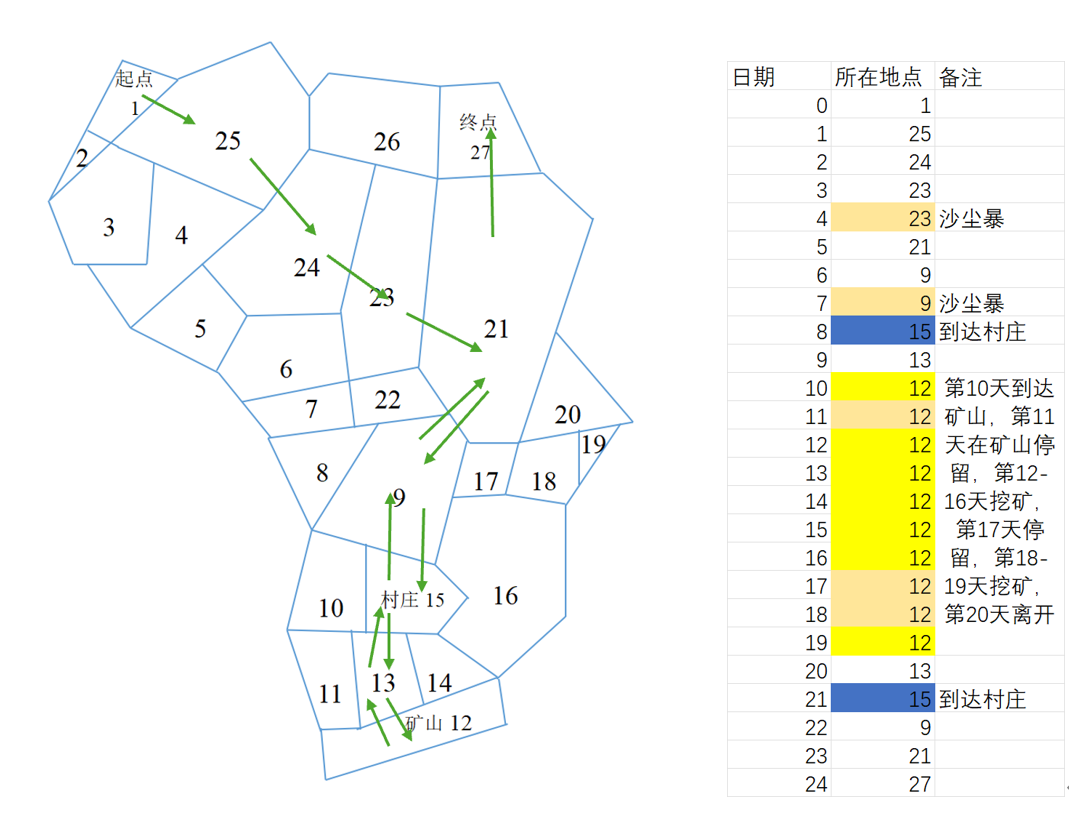
\includegraphics[width=0.8\textwidth]{C2020b/figure/问题一第一关结果图.png}
    \caption{问题一第一关结果图} % 图片标题
\end{figure}

\begin{figure}[H] % 参数 h(here), t(top), b(bottom), p(page) 控制浮动位置
    \centering % 使图片居中
    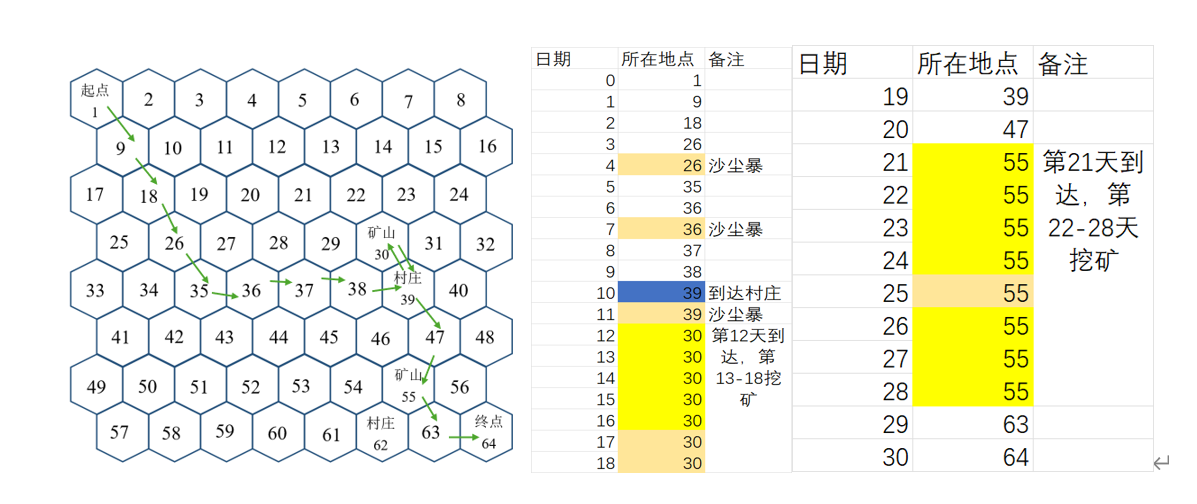
\includegraphics[width=0.8\textwidth]{C2020b/figure/问题一第二关结果图.png}
    \caption{问题一第二关结果图} % 图片标题
\end{figure}

\subsection{问题2的建模和求解}
\subsubsection{模型的建立}
\textbf{1.马尔可夫性质的引入} 

在本题中，因为玩家仅知道当天的天气状况，并需要据此决定当天的行动方案，
%
所以过去的天气对当下已经没有任何参考价值。
%
那么天气随机的限制可简化为在每一天中只知道当前的天气状态，同时通过预测下一天的天气来帮助玩家进行下一步的决策，
%
根据该天气性质，可以引入马尔科夫性来解决此问题：
%
即下一状态只依赖于当前状态，与过去状态无关。以下给出马尔可夫的数学表达式：
\begin{align}
P\bigl(X_{n+1}=x \mid X_1=x_1, X_2=x_2, \dots, X_n=x_n\bigr) = P\bigl(X_{n+1}=x \mid X_n=x_n\bigr)
\end{align}

\textbf{2.引入马尔可夫后的决策过程} 

在玩家决策时，不仅要考虑天气的外部因素，还需要考虑自身负重、行走天数、水和食物等内部因素，
%
不同的未来天气会让玩家做出不同的决策。所以要建立基于马尔可夫性质的决策方程：
\begin{align}
F = \bigl(D_t,~I, ~G_t\bigr)
\end{align}

其中，$D_t$为第t天的天气， $I$为内部因素（包括自身负重、行走天数、水和食物），
%
$G_t$为在$D$这个天气序列下在第t天的剩余资金。

\textbf{3.约束条件的界定} 

在题目中，首先要保证在规定的时间内到达终点，其次才是保留尽可能多的资金。
%
所以我们应该优先考虑能否走到终点。
%
即我们应该在起点买足所有的水和食物，以确保在最坏的天气情况下可以到达村庄或终点来补充物资：
\begin{align}
T_t \geqslant 0, F_t \geqslant 0
\end{align}

其中，$S$为从起点到村庄或终点的路径。

\textbf{4.具有马尔可夫性质的模型总结} 

基于以上分析，我们可写出最后的具有马尔可夫性质的最大化收益决策模型：
\begin{align}
F = \{ F(t) \mid F(t) \text{ 为基于 } (D_t, I) \text{ 算出来的最大化收益} \}
\end{align}

整合即得：
\[
\begin{aligned}
\max_{} \quad & F(t) \\
\text{s.t.} \quad & 0 \le t \le 30, \\
& G_t \ge 0,\; F_t \ge 0,\; T_t \ge 0, \quad t = 0,1,\dots,30, \\
& 0 < M_t \le M_{\max}, \quad t = 0,1,\dots,30, \\
& D_t = 3 \implies N_t = N_{t-1}, \quad t = 1,\dots,30.
\end{aligned}
\]

\subsubsection{模型的求解及结果}

\textbf{动态规划求解} 

\textbf{1.数据初始化}
根据表格数据初始化各天气的食物和水的消耗和路线，设定每个状态的最大收益为无穷小。
%
同时根据第一天的天气给出初始水和食物的购买方案。

\textbf{2.约束条件的补充}

动态规划算法必须当前一步有解才能进行下一步的状态转移，所以我们要确定在不同天气序列下的解的范围。

在每个状态下，都先从最坏的情况下进行考虑，假设后面全部都是高温，从而获得一个能走到终点的结果，
%
即所有解的下界。

\textbf{3.动态规划的求解}

利用跟问题一相同的动态规划算法求解。

\textbf{4.结果线路的输出}

利用dfs回溯法来反向寻找经过路线。

根据以上流程来进行第三关，第四关的求解。

\textbf{结果呈现和分析}

\textbf{1.第三关结果呈现}

由于第三关仅有晴朗和高温两种天气情况，所以我们采用二叉决策树来表现在每一个点上的决策和状态变化。结果如下图。\\

\begin{figure}[H]
    \centering
    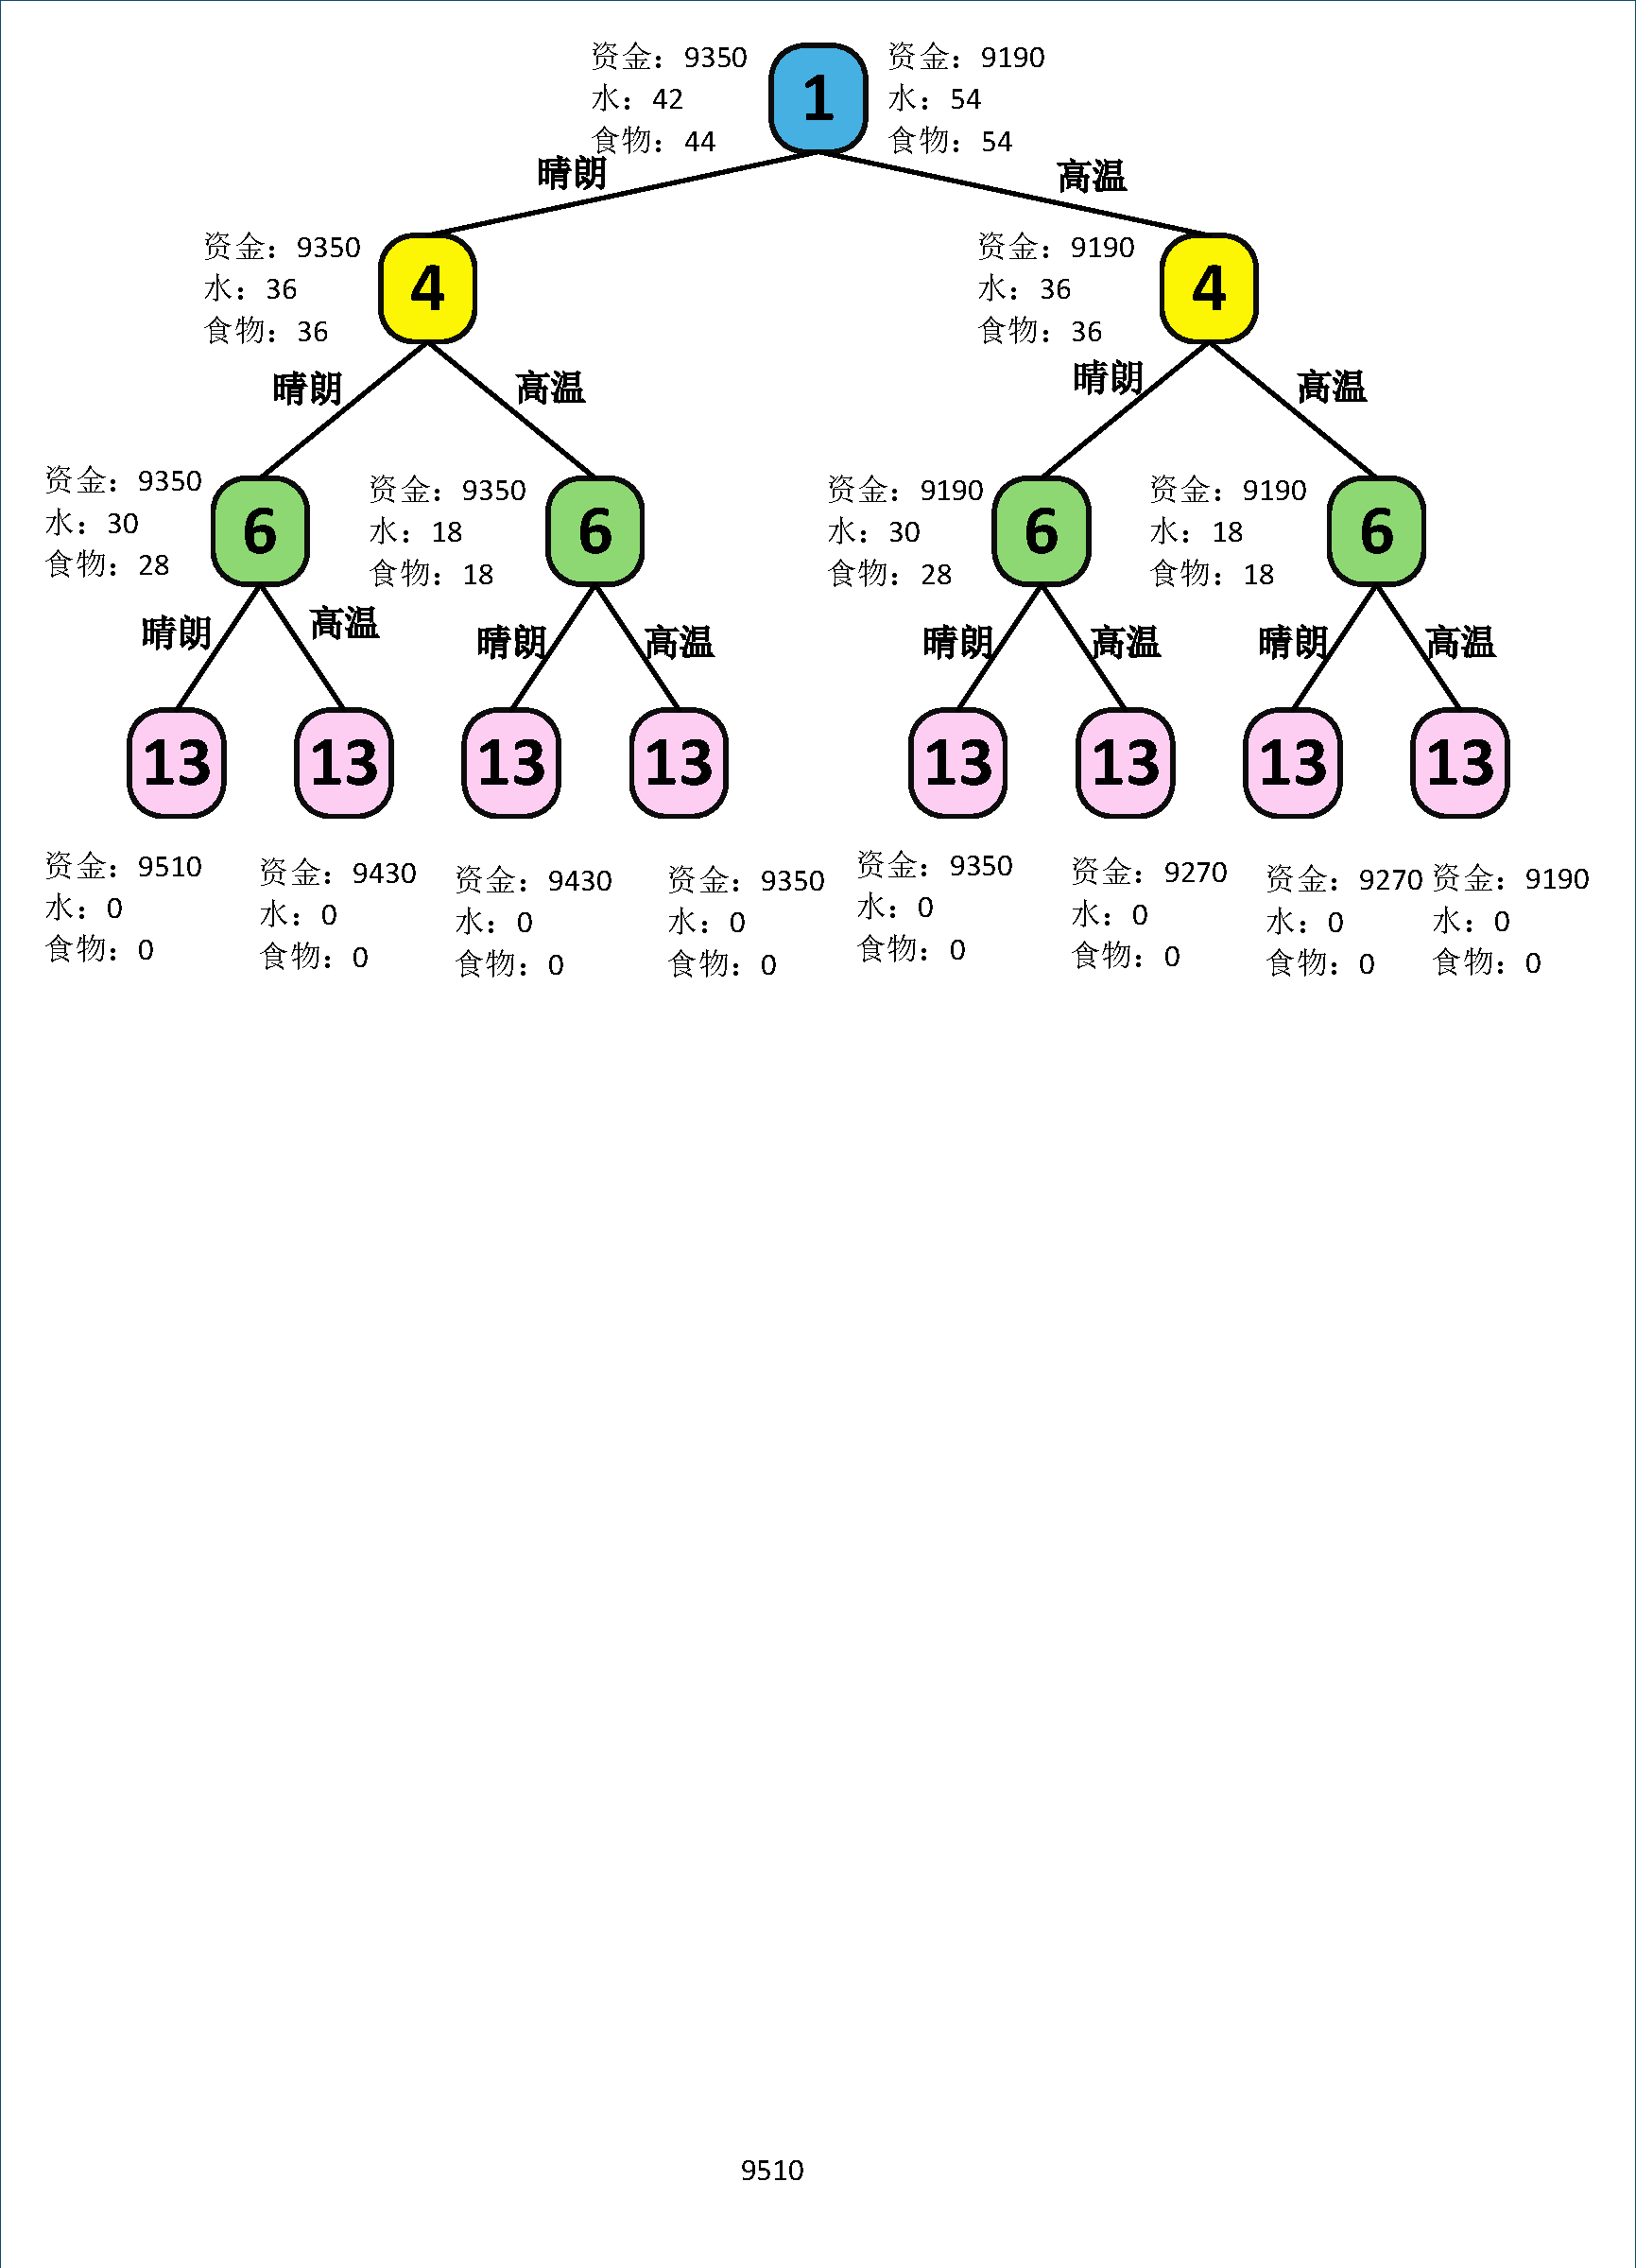
\includegraphics[width=0.8\textwidth]{C2020b/figure/第三关结果图.pdf}
    \caption{第三关结果图}
\end{figure}

我们可以发现路线均是从$1->4->6->13$。说明在该沙漠的地图下，通过如上的决策得到的最优解相同，所以该决策具有稳定性。

\textbf{2.第四关结果呈现}

由于第四关存在晴朗，高温和沙暴三种天气情况，且到终点的最少天数也需要10天，所以使用二叉决策树会使得结果冗余。故采用画图法来展示结果\\

与第三关相同在每个状态下，都先从最坏的情况下进行考虑，假设后面全部都是高温，中间小概率随机插入沙暴天气，从而获得一个能走到终点的结果，即所有解的下界\\

如下是其中一种可能的路线结果：

\begin{figure}[H]
    \centering
    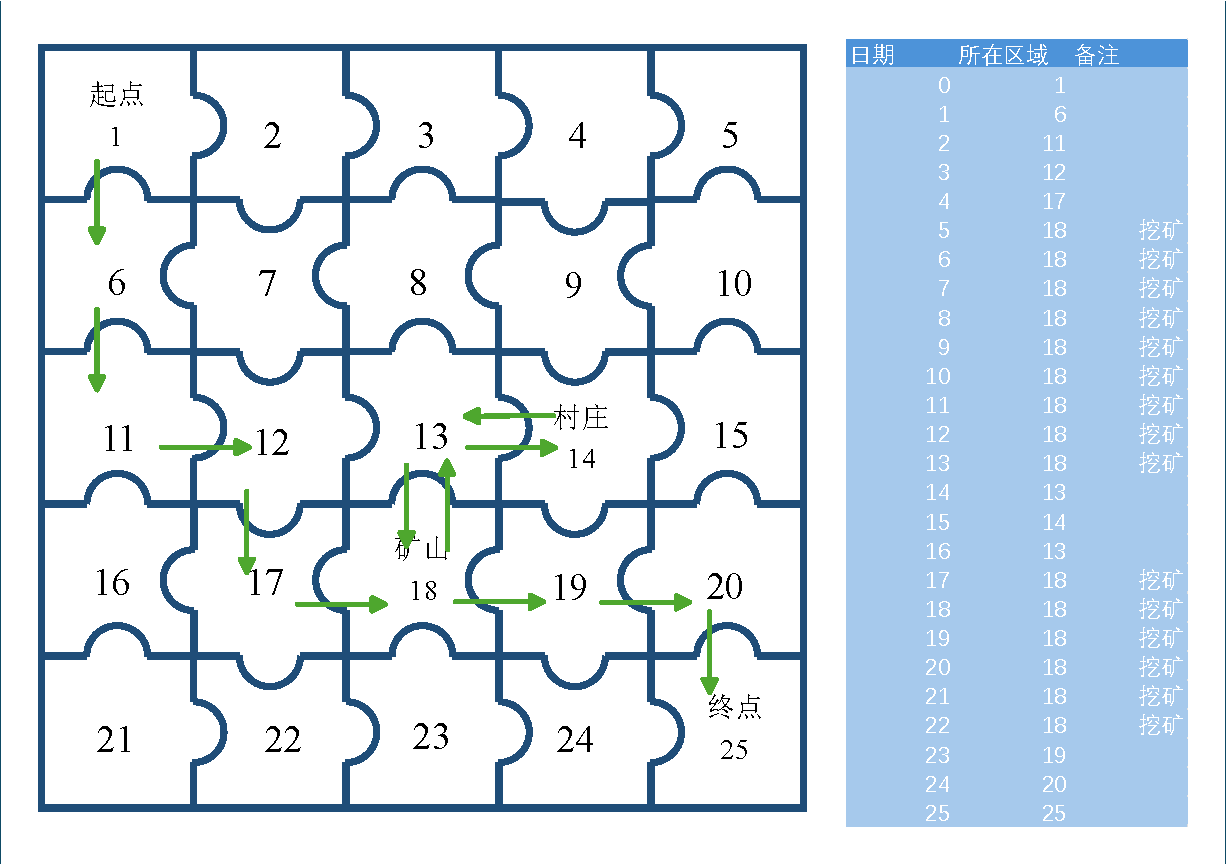
\includegraphics[width=0.8\textwidth]{C2020b/figure/第四关结果图.pdf}
    \caption{第四关结果图}
\end{figure}

所有时刻的各种状态如下：\\

\begin{figure}[h]
\centering
\begin{subfigure}[t]{0.48\textwidth}
\centering
\renewcommand{\arraystretch}{1.2}
\begin{tabular}{|c|c|c|c|c|}
\hline
天数 & 当前位置 & 当前水 & 当前食物 & 利润 \\
\hline
0 & 1 & 196 & 305 & 5970 \\
1 & 6 & 190 & 297 & 5970 \\
2 & 11 & 184 & 289 & 5970 \\
3 & 12 & 178 & 281 & 5970 \\
4 & 17 & 172 & 273 & 5970 \\
5 & 18 & 166 & 265 & 5970 \\
6 & 18 & 157 & 253 & 6970 \\
7 & 18 & 130 & 226 & 7970 \\
8 & 18 & 103 & 199 & 8970 \\
9 & 18 & 94 & 187 & 9970 \\
10 & 18 & 85 & 175 & 10970 \\
11 & 18 & 76 & 163 & 11970 \\
12 & 18 & 67 & 151 & 12970 \\
\hline
\end{tabular}
\end{subfigure}
\hfill
\begin{subfigure}[t]{0.48\textwidth}
\centering
\renewcommand{\arraystretch}{1.2}
\begin{tabular}{|c|c|c|c|c|}
\hline
天数 & 当前位置 & 当前水 & 当前食物 & 利润 \\
\hline
13 & 18 & 40 & 124 & 13970 \\
14 & 13 & 22 & 106 & 14970 \\
15 & 14 & 225 & 225 & 15970 \\
16 & 13 & 219 & 217 & 16970 \\
17 & 18 & 213 & 209 & 17970 \\
18 & 18 & 186 & 182 & 17970 \\
19 & 18 & 159 & 155 & 17710 \\
20 & 18 & 132 & 128 & 16860 \\
21 & 18 & 105 & 101 & 16860 \\
22 & 18 & 96 & 89 & 17860 \\
23 & 19 & 90 & 81 & 17860 \\
24 & 20 & 84 & 73 & 17860 \\
25 & 25 & 78 & 65 & 17860 \\
\hline
\end{tabular}
\end{subfigure}
\end{figure}



\subsection{问题3的建模和求解}
\subsubsection{总述}

前两问分别讨论了单人情形下“已知全程天气”的静态最优策略与“仅知当天天气”的动态最优策略。
%
第三问在此基础上引入多名玩家同时出发的协同决策机制，并在题设中额外加入三类拥挤效应：

\begin{itemize}
    \item 同行惩罚：若某日有多名玩家沿同一边同时移动，则每位玩家的移动消耗按更高倍率计算；
    \item 同矿惩罚：若某日有多名玩家在同一矿山挖矿，则每位玩家的挖矿消耗更高且单位收益下降；
    \item 同购惩罚：若某日有多名玩家在同一村庄同时购买资源，则每箱资源价格上升。
\end{itemize}

因此，第三问已不再是单纯的“最优路径”问题，
%
而是路径选择、出发时机、停留时机、补给时机与挖矿时机的多主体耦合优化问题。
%
本文将前两问的路径模型作为第三问的基础模块，
%
建立“最短路预处理 + 单人可行策略集生成 + 多人协同调度优化 + 未知天气滚动博弈修正”的统一建模框架。

我们可将问题分为两类情形：

\begin{itemize}
    \item 每天气象序列事先已知，各玩家第0天即需确定全程方案，属于静态协同规划问题；
    \item 仅知道当天天气，且每天结束后可观察其他玩家状态并修正次日决策，属于动态协同博弈问题。
\end{itemize}

为统一处理这两类问题，本文将第三问拆解为三个层次：

\begin{itemize}
    \item 路径层：用前两问中“最短路 + 资源可行性判定”模型，
        生成每位玩家从起点到终点、起点到矿山、村庄到矿山、矿山到终点等若干最短或次短候选路径，
        并形成路径库 $\mathcal P_i$。
    \item 调度层：在候选路径库基础上，对不同玩家的出发日期、等待日期、补给日期、挖矿日期进行联合优化，
        以降低拥挤效应造成的额外损失。
    \item 博弈层：在未知天气条件下，结合天气转移概率、剩余资源和他人状态，
        采用滚动时域优化思想动态重规划路径与角色分工。
\end{itemize}

这一本质上是从单人“点到点最优”推广到多人“时空网络上的协调最优”。

\subsubsection{多人资源演化方程}

第 $i$ 名玩家在第 $t$ 日结束后对应负重为

\begin{center}
    $M_{i,t}=m_w T_{i,t}+m_f F_{i,t} \le \max M.$
\end{center}

为统一描述三种天气和三种动作，引入日资源消耗系数、日价格系数和日盈利系数

\begin{center}
    $\alpha(D_t,X_{i,t},\mathbf k_t),\qquad \beta(D_t,X_{i,t},\mathbf k_t)$,
    $\qquad \gamma(D_t,X_{i,t},\mathbf k_t)$.
\end{center}

分别表示第 $t$ 日水与食物的消耗倍率，其中 $\mathbf k_t$ 表示第 $t$ 日的拥挤状态（有多少玩家一起行动）。
%
于是资源递推方程可写为

\begin{center}
    $T_{i,t}=T_{i,t-1}+B_{w,i}(t)-\beta(D_t,X_{i,t},\mathbf k_t)C_w,$
    $F_{i,t}=F_{i,t-1}+B_{f,i}(t)-\beta(D_t,X_{i,t},\mathbf k_t)C_f.$
\end{center}

其中，$B_{w,i}(t),B_{f,i}(t)$ 仅当玩家在起点初始采购或在村庄补给。若玩家未到终点前出现

\begin{center}
    $T_{i,t}<0 \quad \text{或} \quad F_{i,t}<0,$
\end{center}

则判定该策略失效。

资金递推方程为

\begin{center}
    $G_{i,t}=G_{i,t-1}-\Pi_{i,t}^{\text{buy}}+\Pi_{i,t}^{\text{mine}},$
\end{center}

其中 $\Pi_{i,t}^{\text{buy}}$ 为第 $t$ 日购买资源的支出，$\Pi_{i,t}^{\text{mine}}$ 为第 $t$ 日挖矿收益。
%
到达终点后，剩余资源按半价回收，因此玩家最终收益记为

\begin{center}
    $S_i=G_{i,T}+\frac12 P_w T_{i,T}+\frac12 P_f F_{i,T}.$
\end{center}

联盟总收益为

\begin{center}
    $S=\sum_{i=1}^n S_i.$
\end{center}

\subsubsection{拥挤效应的定量刻画}

第三问区别于前两问的关键，在于玩家间相互作用改变了消耗、收益与价格。为此分别刻画三类拥挤效应。

\paragraph{同行惩罚}
移动状态下的资源消耗可统一写为

\begin{center}
    $\beta(D_t,1,\mathbf k_t)=2k_t^{uv}\,\beta_0(D_t,1),$
\end{center}

其中 $\beta_0$ 为单人情况下由天气和动作确定的基础消耗倍率。

\paragraph{同矿惩罚}

根据题意，若多人同矿挖矿，则每人的资源消耗放大，且每人每天获得收益降为基础收益的某一分配比例。
%
对应的消耗倍率写成

\begin{center}
    $\beta(D_t,3,\mathbf k_t)= 3\times\beta_0(D_t,3).$
\end{center}

对应获得的资金倍率以及资金为

\begin{center}
    $\gamma(D_t,3,\mathbf k_t)=  \frac{1}{k_t^h}\times \gamma_0(D_t,3)$,
    $\Pi_{i,t}^{\text{mine}}=\gamma(D_t,3,\mathbf k_t)\times W_0$.
\end{center}

$W_0$为单人挖矿基础收益。当 $k_t^h$ 较大时，虽然联盟总体仍可能因多点挖矿而受益，
%
但单个矿点的边际收益会显著下降，因此“矿山分流”成为多人策略中的核心。

\paragraph{同购惩罚}

令

\begin{center}
    $k_t^v=\sum_{i=1}^n Q_{i,t}^{v}$
\end{center}

表示第 $t$ 日在村庄 $v$ 同时购买资源的玩家数。于是购买成本写为

\begin{center}
    $\Pi_{i,t}^{\text{buy}}=4\times \big[P_w B_{w,i}(t)+P_f B_{f,i}(t)\big].$
\end{center}

该式体现出“同步补给越集中，补给成本越高”，因此在多人情形下应尽量错开采购时间，或将玩家分散到不同补给窗口。

\paragraph{联盟目标函数：收益与稳定性的双目标规划}

若仅以联盟总收益 $G_S$ 为目标，则可能出现“少数玩家获利很高、其余玩家收益很低”的情况；
%
若只追求均分收益，则又可能牺牲整体最优。所以我们确定第三问为收益-稳定性双目标优化问题。

定义联盟稳定性为

\begin{center}
    $\delta =1-\frac{\sqrt{\frac1n\sum_{i=1}^n(G_i-\bar G)^2}}{\bar G+\varepsilon},$
\end{center}

其中 $\varepsilon>0$ 为防止分母为零的极小量。显然，$\delta$ 越接近1，表示各成员收益越均衡，联盟越稳定。

于是第三问的双目标模型可表述为

\begin{center}
    $\max\; G_S=\sum_{i=1}^n G_i,$
    $\max\; \delta.$
\end{center}

考虑实际求解时需将双目标转化为单目标，采用加权求和形式：

\begin{center}
    $\max\; J=\lambda \frac{G_S}{G_{S,r}}+(1-\lambda)\delta,$
    $\qquad 0\le \lambda\le 1.$
\end{center}

其中 $G_{S,r}$ 为单人模型或独立决策模型给出的参考收益上界。$\lambda$为权重。
%
若更强调联盟整体利润，可适当提高 $\lambda$；若更强调协作稳定性，则减小 $\lambda$。

由此，第三问的双目标模型可表述为

\begin{center}
    $\max\; G_S=\sum_{i=1}^n G_i,$
    $\max\; \delta.$
\end{center}

\subsubsection{问题三第五关的分析和求解}

由于第五关地图较为简单，我们直接进行分析和求解。

第五关没有村庄，所以无需考虑补给问题。现已知两特殊节点之间的最短路径（如图第五关示意图）。

\begin{figure}[htbp]
  \centering
  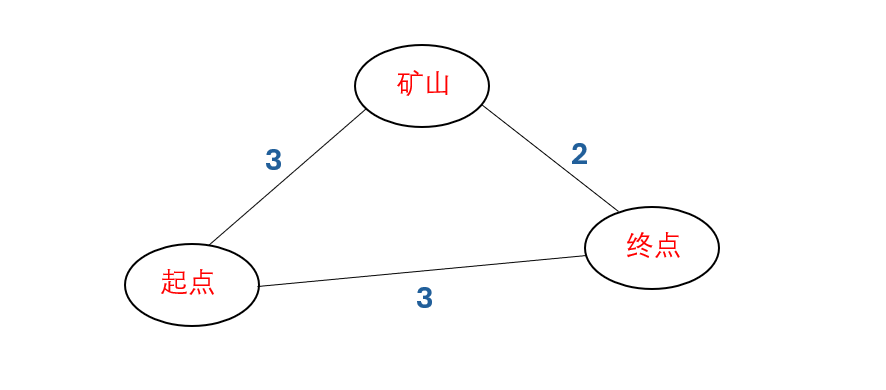
\includegraphics[width=0.5\textwidth]{C2020b/figure/问题三第五关示意图.png}
  \caption{第五关示意图}
\end{figure}

如果玩家决策为去矿山挖矿，那么考虑在矿山的消耗物资的价格为$3\times(3\times5+4\times10)=165元$（晴朗），
%
$3\times(9\times 5+9\times10)=405元$，因此只有晴朗挖矿才可能盈利（最多盈利35元）。
%
加上路上多消耗的两天物资资金至少为$380元$, 而根据天气情况挖矿最多赚$2\times 35=70元$，
%
显然无法实现通过挖矿盈利的目的。

​因此，我们考虑直达终点的情况。
%
直达终点有两条最短路径（1→5→6→13和1→4→6→13），一条备选次短路（1→4→6→12→13）。
%
由于两人一同运动时会消耗4倍基础消耗量，所以应考虑分流。
%
我们分别计算一人走最短路1，一人走次短路（如图第五关分开走示意图所示）和
%
两人分别走两条最短路（如图第五关一起走示意图所示）的最终消耗。
%
其中以蓝色路线为A玩家，橙色路线为B玩家。

\begin{figure}[htbp]
  \centering
  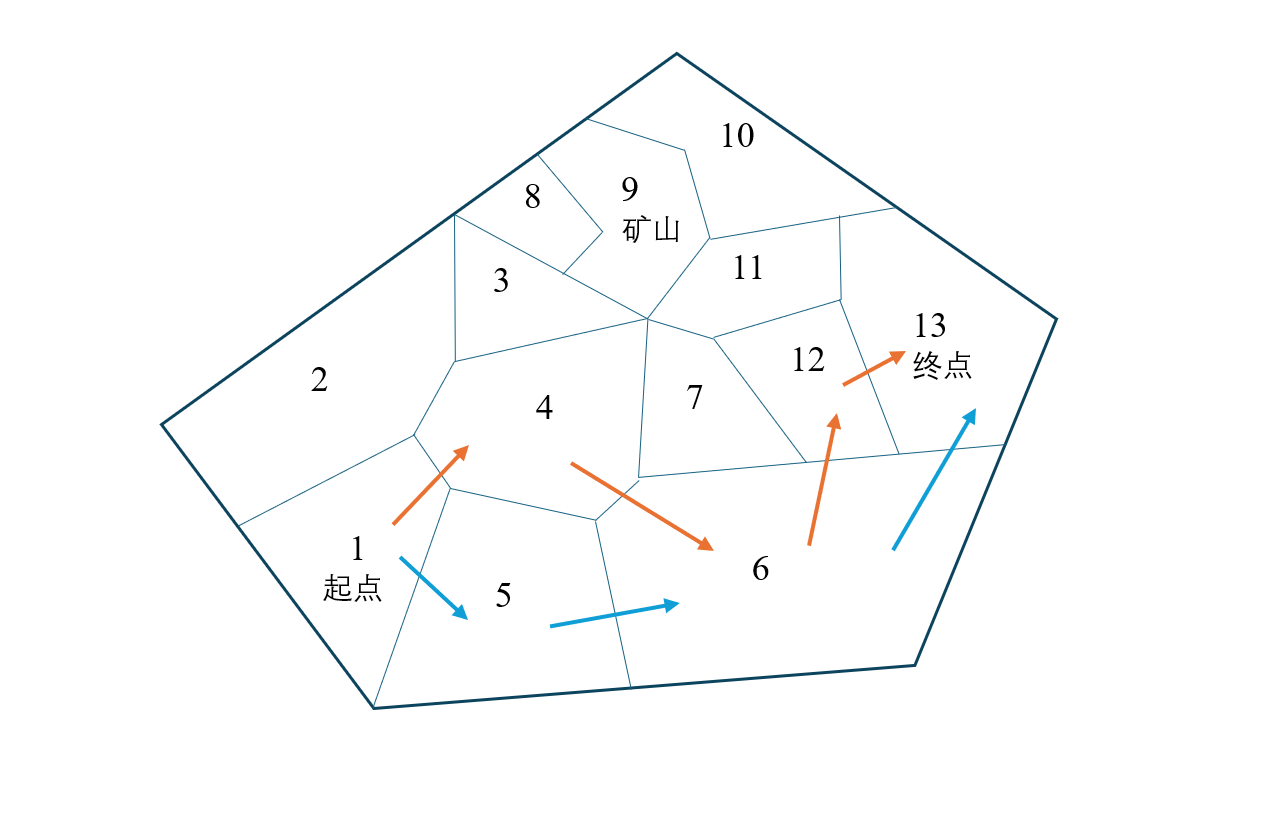
\includegraphics[width=0.5\textwidth]{C2020b/figure/第五关分开走示意图.png}
  \caption{第五关分开走示意图}
\end{figure}

\begin{figure}[htbp]
  \centering
  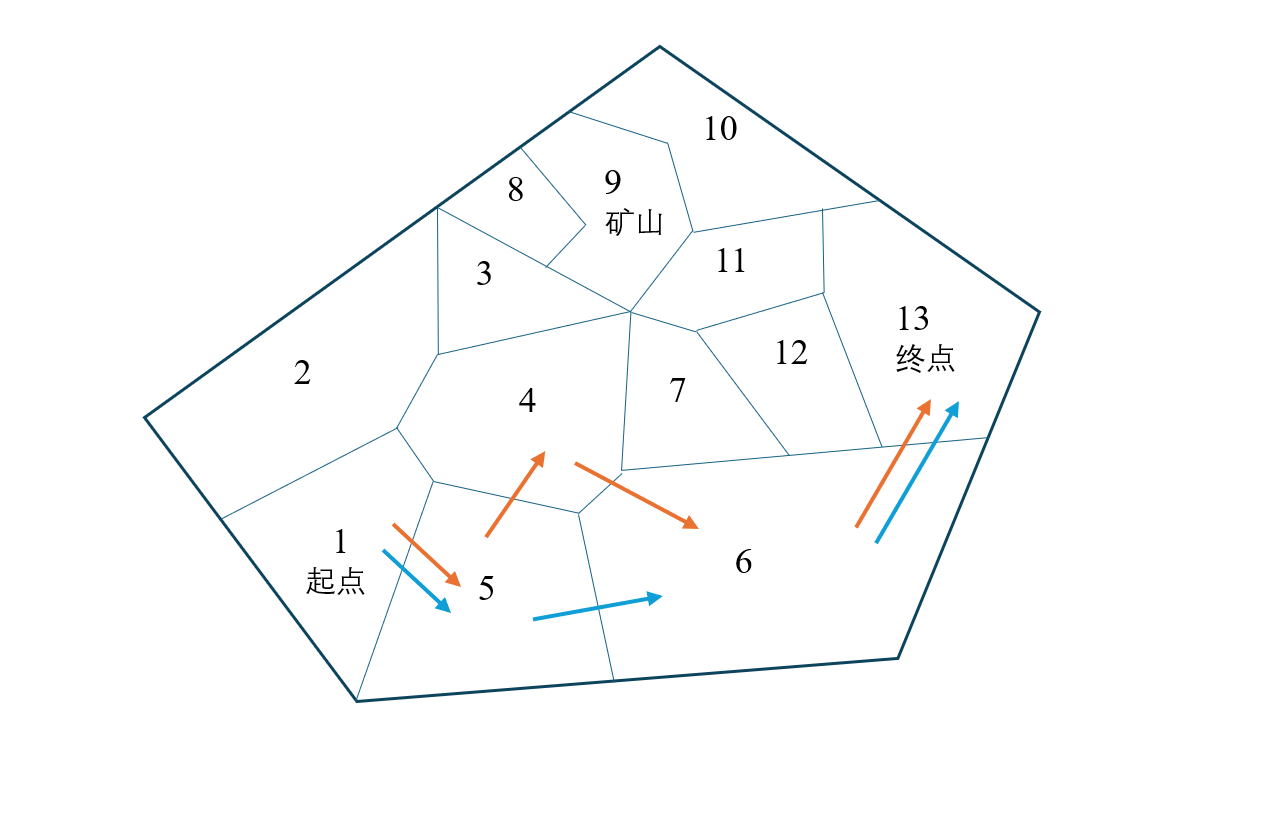
\includegraphics[width=0.5\textwidth]{C2020b/figure/第五关一起走示意图.png}
  \caption{第五关一起走示意图}
\end{figure}

由此可得

\begin{center}
    $490(A)+600(B)=1090元\qquad (\text{图第五关分开走示意图}),$\\
    $600(A=B)\times 2=1200元\qquad(\text{图第五关一起走示意图})$
\end{center}

对于图5关一起走示意图方案进一步优化，为避免第三天两人一起移动，
%
让A玩家在第二天选择停留，即（图第五关优化示意图）。

\begin{figure}[htbp]
  \centering
  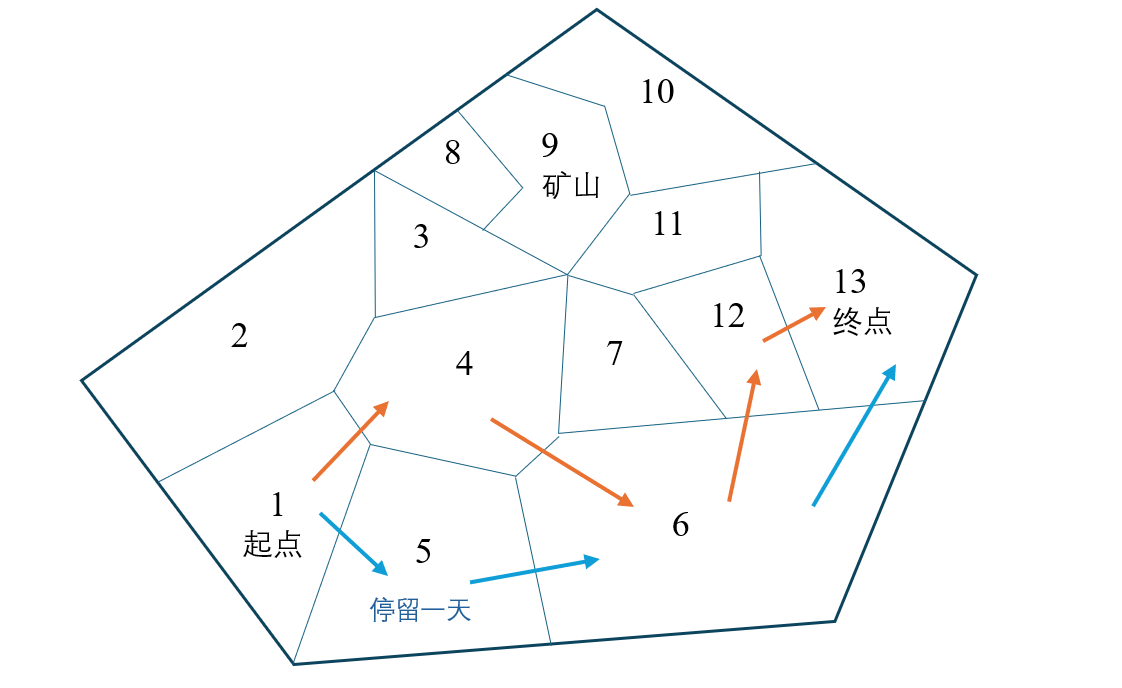
\includegraphics[width=0.5\textwidth]{C2020b/figure/第五关优化示意图.png}
  \caption{第五关优化示意图}
\end{figure}

计算得到最优解

\begin{center}
    $490(A)+465(B)=955元$
\end{center}

因此，最终方案如第五关优化示意图所示。

\subsubsection{第六关求解}

\paragraph{第六关分析}

\subparagraph{天气演化模型}

根据历史天气统计构造转移概率矩阵

\begin{center}
    $
    \mathbf P=
    \begin{pmatrix}
    \pi(1\mid 1) & \pi(2\mid 1) & \pi(3\mid 1)\\
    \pi(1\mid 2) & \pi(2\mid 2) & \pi(3\mid 2)\\
    \pi(1\mid 3) & \pi(2\mid 3) & \pi(3\mid 3)
    \end{pmatrix}.
    $
\end{center}

则在第 $t$ 日已知天气为 $D_t=d$ 时，对未来第 $t+1$ 日天气的预测分布为

\begin{center}
    $
    \mathbb P(D_{t+1}=d'\mid D_t=d)=\pi(d'\mid d).
    $
\end{center}

若需预测未来多日，则可用马尔可夫链幂次转移

\begin{center}
    $
    \mathbb P(D_{t+\tau}=d'\mid D_t=d)=\big(\mathbf P^{\tau}\big)_{dd'}.
    $
\end{center}

这一步将第二问中“依据当天天气滚动修正”的思想进一步形式化。

\subparagraph{状态变量与价值函数}

记第 $t$ 日联盟整体状态为
\begin{center}
    $
    \mathcal X_t=
    \Big(\{N_{i,t}\}_{i=1}^n,\{T_{i,t}\}_{i=1}^n,\{F_{i,t}\}_{i=1}^n,\{G_{i,t}\}_{i=1}^n,D_t\Big).
    $
\end{center}

则联盟在第 $t$ 日的优化目标写为

\begin{center}
    $
    V_t(\mathcal X_t)=\max_{\mathbf u_t}\left\{r_t(\mathcal X_t,\mathbf u_t)+
    \mathbb E\big[V_{t+1}(\mathcal X_{t+1})\mid \mathcal X_t,\mathbf u_t\big]\right\},
    $
\end{center}

其中 $\mathbf u_t$ 表示第 $t$ 日所有玩家的联合动作，$r_t$ 为当日即时回报，
%
包括挖矿收益、补给支出、资源回收价值变化及拥挤损失等。

由于直接求精确动态规划维数过高，本文采用滚动时域近似：每天仅向后预测 $H$ 天，
%
在该短预测窗内求解近似最优联合动作；次日获得新天气和新状态后，再重新规划。
%
这一方法兼顾了计算可行性与策略适应性。

\subparagraph{联盟协同规则}

在动态环境下，多人最优不仅取决于路径，还取决于角色分工。
%
结合前两问可得，玩家在第六关中通常会出现以下三类角色：

\begin{itemize}
    \item 返程优先型：剩余资源偏少且已接近终点，优先采用最短路回终点；
    \item 挖矿收益型：位于矿山附近且资源尚充足，可继续挖矿获取额外收益；
    \item 补给缓冲型：位于村庄附近，用于承担补给和中转功能，避免多人同日同矿或同购。
\end{itemize}

因此，可为联盟制定如下优先级规则：

\begin{itemize}
    \item 若某玩家的安全裕度
          \begin{center}
                $R_{i,t}=\frac{T_{i,t}}{\widehat T_{i,t}^{\text{need}}}+
                \frac{F_{i,t}}{\widehat F_{i,t}^{\text{need}}}$
          \end{center}
          低于阈值 $\theta_1$，则该玩家次日优先返程；
    \item 若某玩家处于矿山附近且预计未来若干日晴朗概率较高，则优先挖矿；
    \item 若预计未来高温或沙暴概率升高，则减少矿山驻留人数，并提前向终点方向收缩；
    \item 若村庄将发生多人同购，则对补给日期进行错峰，控制 $k_t^v$。
\end{itemize}

通过这些规则，可把原本高度耦合的多人策略分解为“少数关键优先级 + 每日局部重规划”的形式。

\paragraph{第六关模型}

第六关中仅知道玩家数目n=3，且天气较少出现沙暴。
%
基于问题二已知这个地图中选择挖矿可获取最大剩余资金。
%
但由于多名玩家同时挖矿会导致挖矿利润骤减，因此可以考虑合作而非竞争的模式。
%
即在满足3人游戏都成功的前提下，只看重集体盈利，个人亏损权重较小。

综合考虑，可得出以下策略：

\begin{itemize}
    \item 让玩家A进行挖矿，玩家B、C选择直达终点（尽量避让同行）；
    \item 为了让三名玩家分流，所以规定挖矿者A走1→6→11→16→17→18（矿山）的行走路线；
    \item 由于与1相接的只有2、6两个模块，因此让B玩家先出发，C玩家原地停留1天后出发（假设当天非沙暴天），
        可选 起点→终点 最短路线行走
\end{itemize}

基于以上分析，我们通过蒙特卡洛算法形成天气预测模型随机模拟天气状况。

因为根据已知，我们知道这里较少出现沙暴，所以控制沙暴天数占总天数的比例$\leq 1/3$, 
%
且对于任意连续 j （j大于等于2）天内，沙暴天数比例$\leq 1/2$的概率在90\%以上。
%
根据非必要不停留的原则，从起点到终点需要移动 8 天，基于以上假设，
%
我们可以得出最坏的情况即移动的 8 天都是高温天，总共路上有  4-10 天沙暴天。
%
玩家消耗资源重量为920kg-1220kg，其中只有10天沙暴天会导致游戏失败，
%
此出现概率大约为1.14\%（假设沙暴天数在剩余10\%概率内平分）。

同理，从起点到村庄的最坏天气状况为 5日高温，3-10日沙暴天。
%
按此计算最多消耗重量为600-950kg 资源因此，玩家存活到达村庄的概率是100\%。

对于一部分玩家，出于心理因素，会在村庄进行物资补给，以保证游戏100\%的成功率。
%
但对于n=3的小基数玩家，我们建议无需补给物资。

对于挖矿者，根据问题二的分析，由于挖矿产生消耗，物资不够的概率较大，因此考虑去村庄补给。
%
去村庄需要消耗至少4天，因此若补给次数过多必然会使挖矿天数减少。
%
我们模拟了村庄补给次数与挖矿盈利（挖矿所得-采购资源所耗资金）以及挖矿天数的关系，
%
结果见去村庄补给次数与最大盈利的关系图和去村庄补给次数与最优挖矿天数的关系图。
%
（半数是只从矿山挖矿后去村庄补给，并不返回矿山而直达终点）

\begin{figure}[htbp]
  \centering
  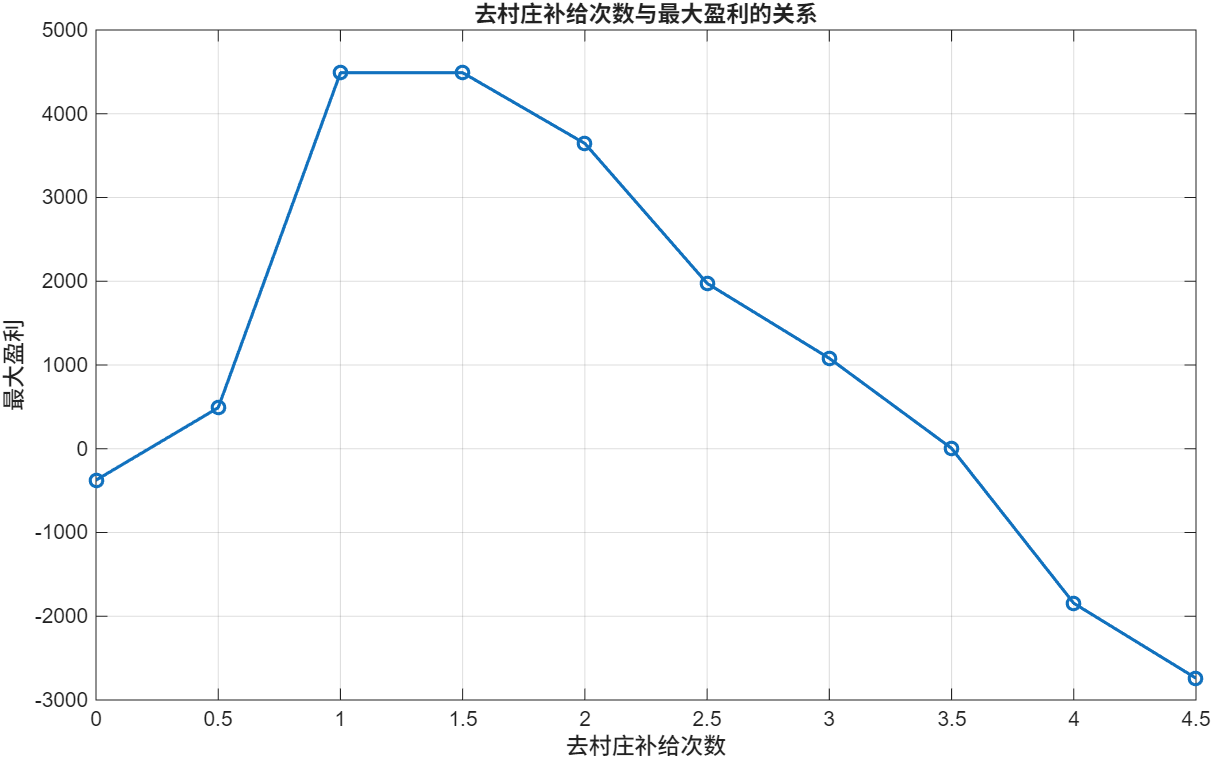
\includegraphics[width=0.5\textwidth]{C2020b/figure/去村庄补给次数与最大盈利的关系图.png}
  \caption{去村庄补给次数与最大盈利的关系图}
\end{figure}

\begin{figure}[htbp]
  \centering
  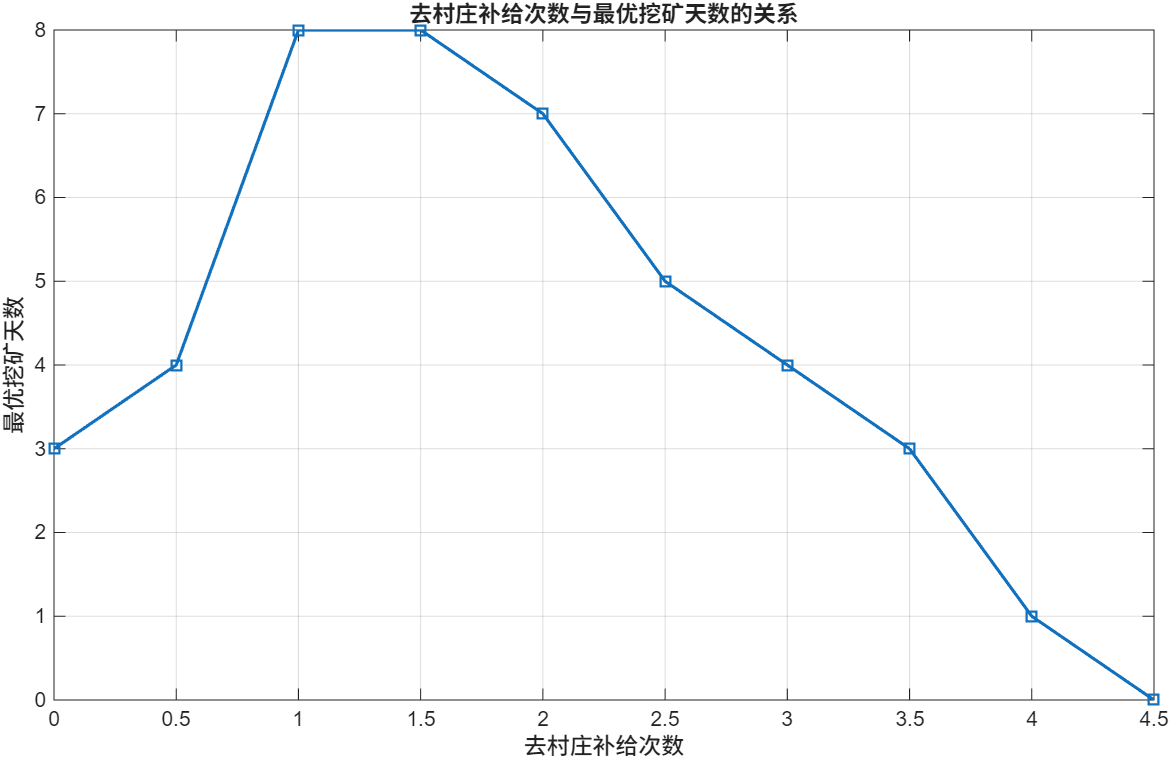
\includegraphics[width=0.5\textwidth]{C2020b/figure/去村庄补给次数与最优挖矿天数的关系图.png}
  \caption{去村庄补给次数与最优挖矿天数的关系图}
\end{figure}

由以上分析，可得出一般情况下的最优路线图（见图第六关一般情况下最优路线图）。

\begin{figure}[htbp]
  \centering
  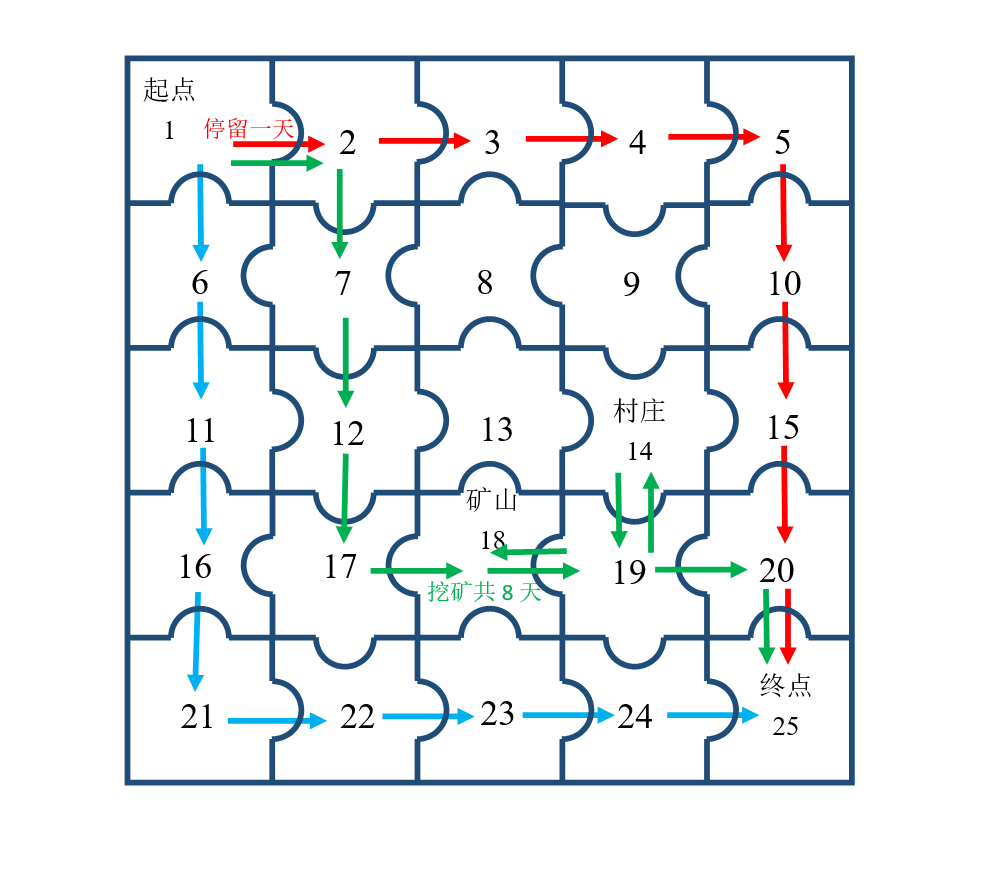
\includegraphics[width=0.5\textwidth]{C2020b/figure/第六关一般情况下最优路线图.png}
  \caption{第六关一般情况下最优路线图}
\end{figure}


\section{模型的评价与改进}
\subsection{模型评价}
\subsubsection{优势}

\subsubsection{局限性}

\subsection{模型改进}

\bibliographystyle{plain}
\bibliography{C2020b/main}

\begin{center}
    \Large\textbf{附录：程序代码}
\end{center}

\begin{minted}{python}

\end{minted}
\end{document}